\chapter{GEVP method}
\label{apex_GEVP}

For the extraction of meson masses involving heavy quark flavors (see Sec.~\ref{ch_charm}), we employ a generalized eigenvalue problem (GEVP) variational method defined as 
\begin{equation}\label{eq:gevp_sec3}
 	\mathit{\mathbb{C}}_X(t) v_n(t,t_{\mathrm{ref}}) = \lambda_n(t,t_{\mathrm{ref}}) \mathit{\mathbb{C}}_X(t_{\mathrm{ref}})v_n(t,t_{\mathrm{ref}}) \qquad n=0,\ldots,N-1 ,
\end{equation}
with $t>t_{\mathrm{ref}}$ and where $\mathit{\mathbb{C}}(t)_X$ is a $N\times N$ matrix of Euclidean correlation functions $C_X$. In particular we use
\begin{equation}
 	\mathit{\mathbb{C}}_{P}(t) = \left(\begin{matrix}
 		C_{P}(t)  &  C_{P}(t+\tau)
 		\\
 		C_{P}(t+\tau)  & C_{P}(t+2\tau)
 	\end{matrix}\right) \,,
\label{eq:gevp_matrix}
\end{equation}
where $C_P(t)\equiv C_P(t+y_0,y_0)$, $t=x_0-y_0$ and $\tau$ is the value of the time shift. Several values of the time shift have been tested, and we observe a mild dependence on small values of $\tau$ for the extraction of eigenvalues and eigenvectors. Specifically, the value $\tau=3a$ was selected. The GEVP  is solved in the regime  $t_{\mathrm{ref}} \geq t/2$, where a better control over excited state contributions is achieved \cite{Blossier:2009kd}. We refer to~\citep{charm} for a detailed discussion of our setup, together with sanity checks on the GEVP. The ground state meson mass $m$ is extracted from the eigenvalues of the GEVP using 
\begin{equation}\label{eq:eff_en_gevp}
	am_{\mathrm{eff}}(t,t_{\mathrm{ref}})=\log\bigg(\frac{\lambda_0(t,t_{\mathrm{ref}})}{\lambda_0(t+a,t_{\mathrm{ref}})}\bigg).
\end{equation}
An example of a GEVP plateau for the heavy-light pseudoscalar mass is shown in Figure \ref{fig:meff_plateau}. 
 
In the case of meson decay constants involving heavy quarks (see Sec.~\ref{ch_charm}), we employ again the GEVP method to extract the ground state signal of the matrix element $ \langle 0 | P^{ij} | P^{ij}(\mathbf{p=0})\rangle $. This is done by considering the normalized eigenvector $v_n(t,t_{\mathrm{ref}})$ in eq.~(\ref{eq:gevp_sec3}),
where $| P^{ij}(\mathbf{p=0})\rangle$ stands for the ground state of the meson with flavor content $i,j$.  Namely, we define for each state $n$ the number \cite{Blossier:2009kd}
\begin{equation}
	R_n = \left(v_n(t,t_{\mathrm{ref}}),\mathit{\mathbb{C}}_{P}(t)v_n(t,t_{\mathrm{ref}})\right)^{-1/2} e^{E_nt/2},
	\label{eq:gevp_effective_operator}
\end{equation}
where $(\cdot, \cdot)$ is the usual scalar product and $\mathit{\mathbb{C}}_{P}$ is the GEVP matrix from eq.~(\ref{eq:gevp_matrix}).  Then, the ground state matrix element is given by
\begin{equation}
	p_{\mathrm{eff}}(t,t_{\mathrm{ref}}) = (v_0(t,t_{\mathrm{ref}}), C_{P,0}) R_0, \qquad (C_{P,0})_k = (\mathit{\mathbb{C}}_{P})_{k0} 
	\label{eq:effective_matrix_element}
\end{equation}
The large distance behavior of the effective matrix element is governed by 
\begin{equation}
	p_{\mathrm{eff}}(t,t_{\mathrm{ref}}) = p_0 + \mbox{O}(e^{-(E_{N+1}-E_0) t_{\mathrm{ref}}}), \qquad p_0 =  \langle 0 | P^{ij} | P^{ij}(\mathbf{p=0})\rangle,
\end{equation}
in the regime where the condition $t_{\mathrm{ref}}\geq t/2$ is satisfied, where $E_0$ is the ground state meson mass. In Figure \ref{fig:decay_plateau} we show a representative plateau for a heavy-light decay constant.

\begin{figure}
  	\centering
  	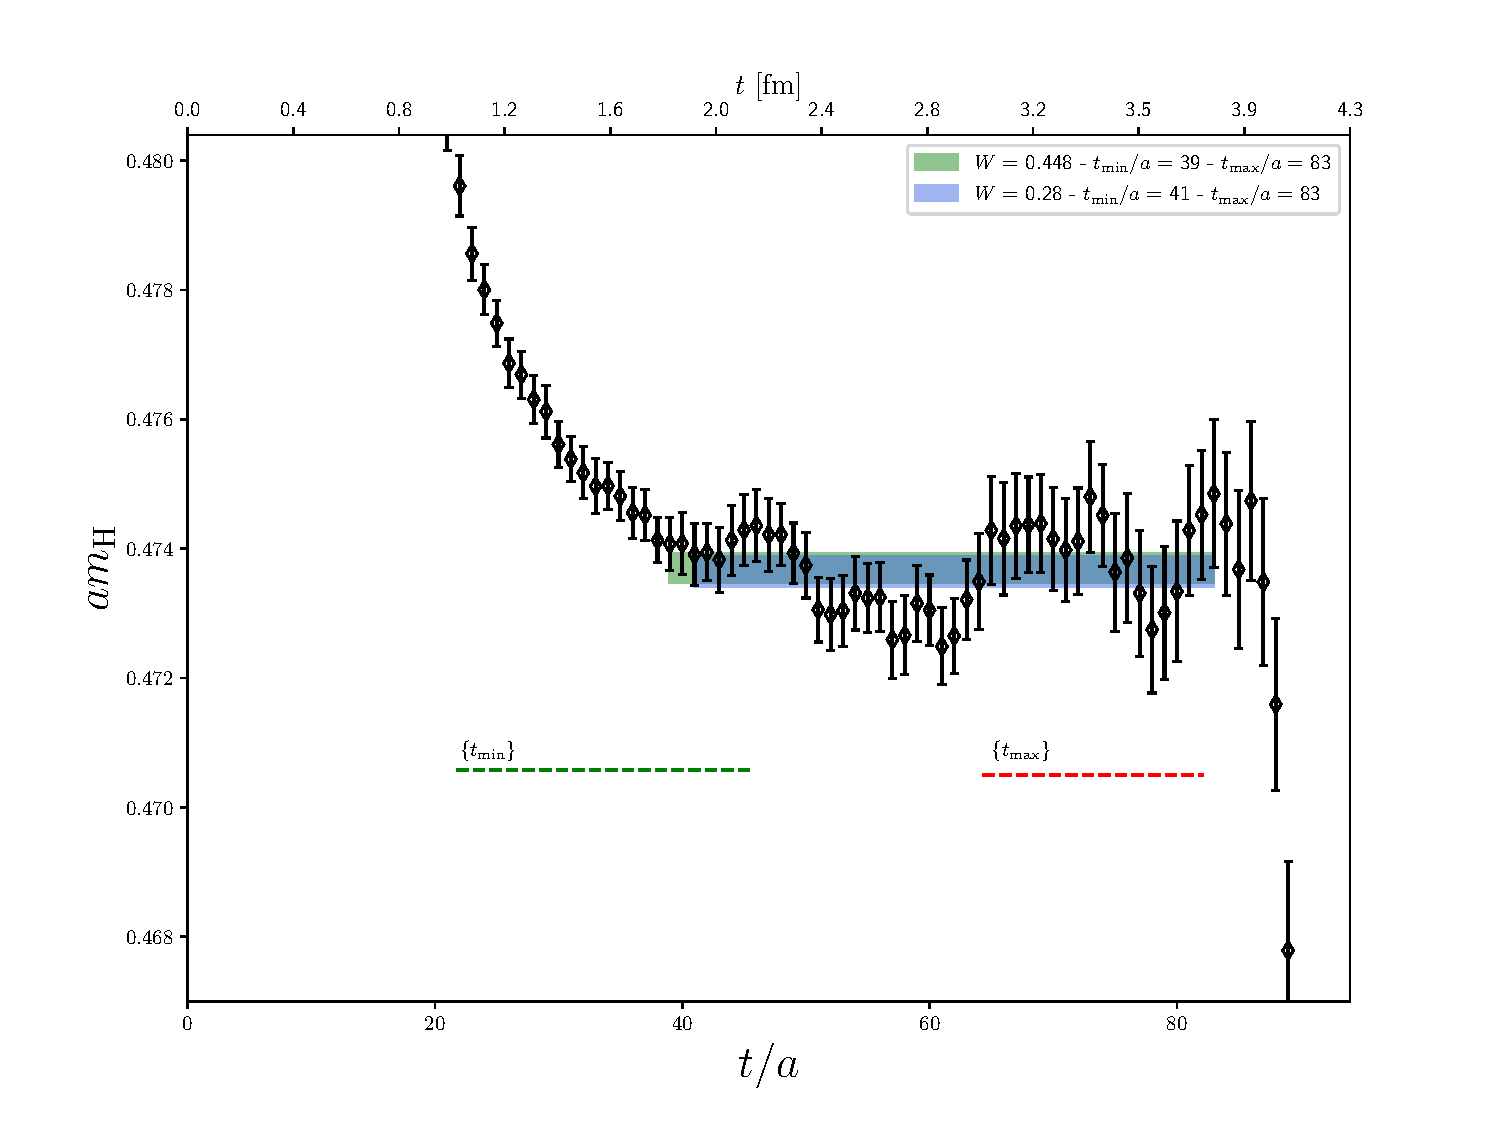
\includegraphics[scale=0.5]{./cap6/figs/matching/m8_plateau.pdf}
  	\caption{Illustration of the extraction of the ground-state mass after applying a GEVP analysis, illustrated for the ensemble J303. We show the heavy-light pseudoscalar meson mass plateau with the two fit intervals with higher weights $W$ contributing to the model average introduced in Sec.~\ref{ch_observables:sec:MA}. We also indicate the range of variations allowed for the interval in Euclidean time where the plateau is taken. The shaded blue and green bands corresponds to two specific plateau choices.} 
\label{fig:meff_plateau} 
\end{figure}

\begin{figure}
	\centering
	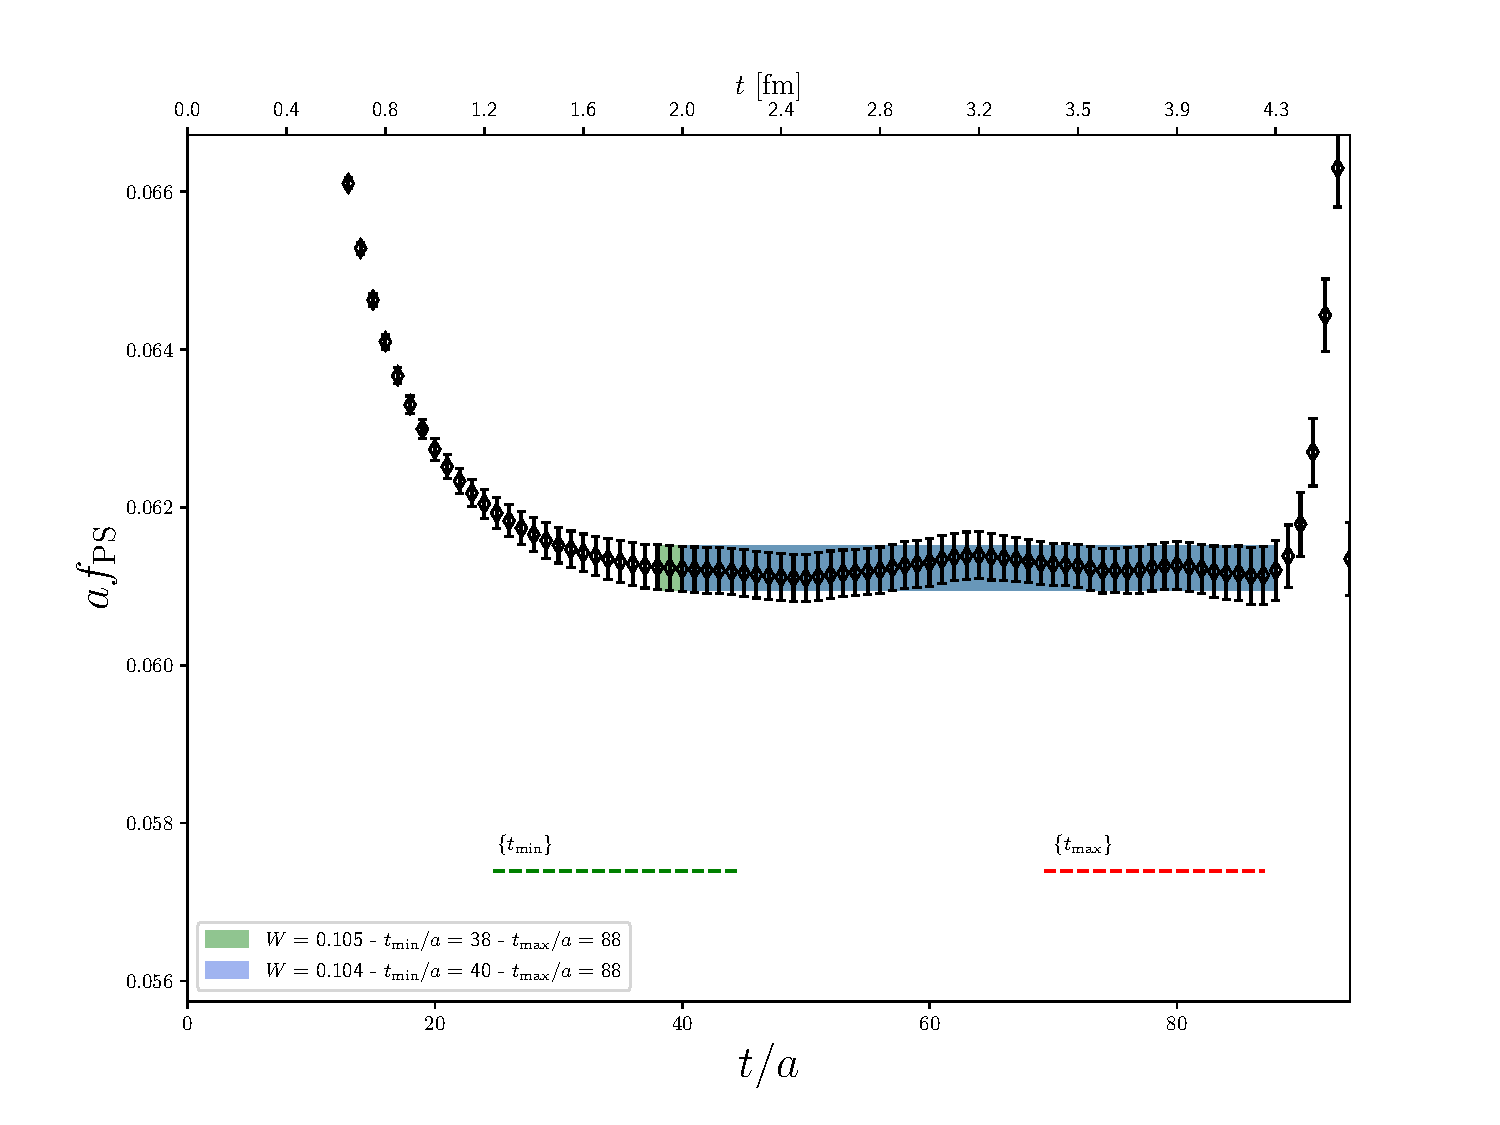
\includegraphics[scale=0.5]{./cap6/figs/fds/f8_plateau.pdf}
	\caption{Illustration of the extraction of the heavy-light pseudoscalar decay constants, after applying a GEVP analysis, for ensemble J303. We show the plateau for the heavy-light pseudoscalar decay constant for the two fit intervals with higher weights in the model average introduced in Sec.~\ref{ch_observables:sec:MA}. The shaded blue and green bands corresponds to two specific plateau choices. }
	\label{fig:decay_plateau} 
\end{figure}